\documentclass{beamer}
\title{Project \& Training 3: Networking Project}
%\subtitle{SUBTITLE}
\date{KW 47/2023}
\author{Hansj\"urg Wenger \& Christian Grothoff}
\institute{Berner Fachhochschule}

\begin{document}

\begin{frame}
  \maketitle
\end{frame}

\begin{frame}{Agenda}
\tableofcontents
\end{frame}

\section{Lab overview}

\begin{frame}{Networking project}
There are three main sprints:
\begin{enumerate}
\item Implement an Ethernet switch
\item Implement the ARP protocol
\item Implement an IPv4 router
\end{enumerate}
Today, we will implement a {\tt hub}, which serves as a quick warm-up.
The {\tt switch} is {\bf not required} for students in BTI 3022.
\end{frame}


\begin{frame}{Networking project: repeating students}

There are {\bf special rules} for students who failed the course previously:
\begin{enumerate}
\item Only one project: {\bf vswitch}
\item Special team size: {\bf two students max}
\item Different passing threshold: {\bf 24 points (team of 2), 20 points (team of 1)}
\item Only one deadline: {\bf same as Sprint 3 for regular students}
\end{enumerate}

\end{frame}


\section{Organization}
\begin{frame}{Team}
  {\bf Suggested} are teams of 4 students.
  This is a {\em suggestion}, not a requirement!
  If your team is smaller, the required thresholds for passing the
  course will be reduced.

  Teams have been pre-assigned, if there are problems
  within your team, do talk to the professors who will
  try to find a solution.
\end{frame}


\begin{frame}{Process}
Three 2-week sprints:
\begin{itemize}
\item Plan algorithms, data structures and testing
\item Implement
\item Unit-test
\item Integration test
\item[$\Rightarrow$] Version in Git at submission time is graded!
\end{itemize}
\end{frame}


\section{Hardware}

\begin{frame}[fragile]{Virtual Hardware}
  \vfill
  \begin{center}
    \url{https://gitlab.ti.bfh.ch/demos/vlab}
  \end{center}
  \vfill
  \begin{center}
    Username: root, password: (given via Mumble) %lab\$mast3r
  \end{center}
  \vfill
{\tiny
\begin{verbatim}
# ./network-driver ens4 ens5 ens6 ens7 - ./switch ens4 ens5 ens6 ens7
\end{verbatim}
}
\end{frame}


\begin{frame}{Hardware}
\begin{itemize}
\item There are two custom USB-to-4x-Ethernet adapters for each
      team in the lab.
\item Please
      add your name to the list with the number of the adapter taken.
\item Also take single USB-Ethernet adapters if your notebook/PC
      does not have an Ethernet port. You may also take an
      Ethernet cable if needed.
\item You must bring everything back after the final submission
      deadline. When you have returned the adapter, you may cross your
      name off the list again.
\end{itemize}
\end{frame}



\begin{frame}{Suggested setup}
\begin{center}
\includegraphics[width=0.7\textwidth]{arch.pdf}
\end{center}
\end{frame}


\section{Software}

\begin{frame}{Skeleton}
Your Gitlab team repository should have been provisioned with a skeleton
that is a starting point. It includes:
\begin{description}
\item[hub.c] Template for the {\tt hub} project. Add 3 lines to get a working hub!
\item[switch.c] Template for the {\tt switch} project.
\item[arp.c] Template for the {\tt arp} project.
\item[router.c] Template for the {\tt router} project.
\item[Makefile] Build system.  Modify as needed.
\item[network-driver.c] Completed driver to allow you to send and receive
   Ethernet frames. You do not need to modify this code!
\end{description}
\end{frame}


\begin{frame}[fragile]{Running the network-driver}
\begin{itemize}
\item LAN driver provided in C in Git ({\tt glab/network-driver.c})
\item Launch driver with list of names of physical network device (i.e. ``lan0'')
      followed by ``-'' followed by the command to run your program:
\begin{verbatim}
  $ sudo network-driver eth0 eth1 eth2 - ./my-hub eth0 eth1 eth2
\end{verbatim}
  The network devices MUST be passed twice: once to the network-driver
  as arguments, and once to your program ({\tt hub}, {\tt switch}, {\tt arp}, {\tt router})!
\item Driver will pass received frames to your {\tt stdin}
\item Driver will read frames from your {\tt stdout} and pass to network
\item Driver will not touch {\tt stderr}, you can use {\tt stderr} for logging
\item Terminate driver via signal (kill) or closing {\tt stdout}
\end{itemize}
\begin{center}
{\bf Your} code can be in {\em any} language!
\end{center}
\end{frame}


\begin{frame}{The Driver I/O Format}
\begin{itemize}
\item First 6 bytes written by driver to your {\tt stdin} are the HW MACs
      for each of the network interfaces (in the same order).
\item Henceforth, the message format is 16-bit length prefix (in big endian),
      followed by 16-bit interface identifier,
      followed by Ethernet frame (destination MAC, source MAC, etc.).
\item To send frames, also use 16-bit length prefix followed
      16-bit interface identifier, followed by Ethernet frame.
\item Interace number 0 is {\bf reserved} for interacting with the console.
\item You must set the source MAC correctly (in particular for {\tt arp}/{\tt router})!
\item Some hardware may not support using source MACs other than your
      HW MAC. If you do not use the provided equipment, check that you have
      hardware that supports sending with arbitrary MACs!
\end{itemize}
\end{frame}


\begin{frame}{Skeleton: Helper files}
Other code in the Gitlab team repository:
\begin{description}
\item[loop.c] Shared logic for all programs. Functions you may use, but
   do not need to modify.
\item[print.c] Replacement for {\tt printf()} given that {\tt stdout}
   is for Ethernet frames and MUST NOT be used for program output.
\item[crc.c] Internet checksum. Feel free to use.
\item[glab.h] Packet format for the interaction with the network-driver.
\end{description}
You do NOT have to modify this code, but it may be useful to understand
it. You MUST re-implement this logic if your project is in languages
other than C.
\end{frame}


\section{Strategy}

\begin{frame}{Suggested Strategy}
\begin{itemize}
\item Understand what a hub/switch/arp/router really has to do.
\item Plan your data structures first. The algorithms are always trivial.
      Use simple tables (except for routing).\footnote{Until the {\tt router},
      you do not need {\tt malloc()} at all!}
\item For testing, write a program that pretends to be the network driver.
      Remember the {\tt shell} project from CS Basics. Use {\tt dup}, {\tt fork}
      and {\tt exec} to run your main program with {\tt stdin}/{\tt stdout}
      being controlled by your test harness.\footnote{{\tt java.lang.ProcessBuilder}
      can also be used.}
\item Perform compatibility tests with real hardware once above tests work.
\end{itemize}
Tests and main program do {\bf not} have to be in the same language.
\end{frame}


\begin{frame}{Test requirements}
  The quality of your tests will {\bf also} be graded.
  \begin{itemize}
  \item Make sure your tests are run via the {\tt make check-XXX} target(s).
  \item The tests should succeed by returning 0, and fail with non-zero.
  \item {\tt make check-XXX} MUST NOT create binaries like {\tt switch}, {\tt arp}
    or {\tt router}.
  \item If you write unit tests for individual functions, please put them
    under a different target, like {\tt make tests}.  Those will NOT be
    graded.
  \end{itemize}
  Why? We will run your test suite against our reference implementation
  as well as buggy implementations!
\end{frame}


\begin{frame}{Grading of your code}
  \begin{itemize}
  \item If you code does not compile with {\tt make}: 0 points. No discussions.
  \item If you code exhibits undefined behavior and thus works on your system
        but not ours: 0 points. No discussions.
  \item We run tests against your
    implementation.  Passing our tests gets you points.
  \item We run your test suite against our correct and
    buggy ({\tt bugX-XXX}) implementations
    --- you get points if your test suite finds our bugs {\bf while passing our
      correct reference implementation}. Bonus points will be awarded for teams
    that find previously unknown bugs in the reference implementation within
    the scope of the specification.\footnote{Contact
      us, if we confirm it is a bug in the reference implementation,
      you get your bonus.}
  \item Test your tests against the provided correct and buggy reference
    implementations!
  \end{itemize}
\end{frame}


\begin{frame}[fragile]{Test starting point}
\begin{verbatim}
int meta (int argc, char **argv) {
  int cin[2], cout[2]; pipe (cin); pipe (cout);
  if (0 == (chld = fork ()) {
    close (STDIN_FILENO); close (STDOUT_FILENO);
    close (cin[1]); close (cout[0]);
    dup2 (cin[0], STDIN_FILENO);
    dup2 (cout[1], STDOUT_FILENO);
    execvp (argv[0], argv);
    printf (stderr, "Failed to run binary `%s'\n", argv[0]);
    exit (1);
  }
  close (cin[0]); close (cout[1]);
  child_stdin = cin[1]; child_stdout = cout[0];
  // send MACs, run test, cleanup
  kill (chld, SIGKILL);
}
\end{verbatim}

\end{frame}

\section{Tools}

\begin{frame}{Git}
The slides and other materials related to the lecture and the project
are on \url{https://gitlab.bfh.ch/}. You should have obtained the links from
the official Moodle page of the course.

You must also use Git for your software development. Make sure to only
share the GitLab repository with your team and the professors. You are
responsible that your solution is only submitted by your team.

When you have questions about your code, it is helpful if the current
version of the code is available to the professor on GitLab for
inspection.
\end{frame}


\begin{frame}{Jitsi}

Init7 hosts a public Jitsi server at {\bf meet.zrh.init7.ch} which you
can use for voice conferencing, including interactive help with the
project. The server is running 24/7, so you are welcome to use it at
any time.

Jitsi can be used to record sessions. You MUST have the consent
of everyone in the room before recording. Lectures MUST NEVER be
recorded.
\end{frame}

\begin{frame}{Scheduling a session}

To receive support via Jitsi, you must first send an e-mail to the
respective instructor asking for help.  Support will be provided only
during the official support period.  The instructor will reply with a
URL and time.
\vfill

You may ask on the day itself.
\vfill

\end{frame}


\end{document}
